\section{Auswertung}
\label{sec:Auswertung}
\subsection{Bestimmung der Dichte}
Um die nachfolgend berechneten Elastizitätsmoduln mit Literaturwerten vergleichen
zu können, wird zunächst die Dichte der Stäbe bestimmt. Mit Hilfe einer Tabelle
wird dann das Metall oder die Legierung bestimmt.
Für Stab 1, der eine quadratische Querschnittsfläche hat, wurden folgende
geometrische Abmessungen bestimmt:
\begin{align*}
  \text{Länge } l_1 &= \SI{0.60}{\meter}\\
  \text{Breite } a &= \SI{0.01}{\meter}\\
  \text{Masse } m_1 &= \SI{0.5025}{\kilo\gram}.\\
  \intertext{Für Stab 2 mit einer runden Querschnittsfläche wurde}
  \text{Länge } l_2 &= \SI{0.60}{\meter}\\
  \text{Durchmesser } d &= \SI{0.01}{\meter}\\
  \text{Masse } m_2 &= \SI{0.5025}{\kilo\gram}
\end{align*}
gemessen. Alle Messungen wurden dabei zehn Mal durchgeführt, um den Fehler des
Mittelwerts bestimmen zu können, da jedoch immer der gleiche Wert gemessen wurde,
ist der Fehler 0.
Die Dichte der Probestäbe wird mit
\begin{equation}
  \rho = \frac{m}{V}
  \label{eqn:dichte}
\end{equation}
bestimmt.
Für die gemessene Dichte des quadratischen Stabes folgt
\begin{equation*}
  \rho_1 = \frac{m_1}{l_1 a^2} = \frac{\SI{0.5025}{\kilo\gram}}{\SI{0.60}{\meter}
  (\SI{0.01}{\meter})^2} = \SI{8375}{\kilo\gram \per \cubic\meter}
  \label{eqn:dichte_stab1}
\end{equation*}
und für die des runden Stabes
\begin{equation*}
  \rho_2 = \frac{m_2}{\pi \left(\frac{d}{2}\right)^2 l_2}
  = \frac{\SI{0.3605}{\kilo\gram}}{\pi \left(\SI{0.005}{\meter}\right)^2 \SI{0.55}{\meter}}
  = \SI{8346}{\kilo\gram \per \cubic\meter}.
  \label{eqn:dichte_stab2}
\end{equation*}

Dies entspricht im Rahmen der relativen Fehler von $\Delta \rho_1 = \SI{0.3}{\percent}$
und $\Delta \rho_2 = \SI{0.6}{\percent}$ der literaturbekannten Dichte von Messing
(\cite[274]{geschke}, Tabelle 1: Einige Eigenschaften fester Stoffe) und legt nahe,
dass die Stäbe aus Messing sind. Für eine Messing-Legierung mit einer Zusammensetzung
von $\SI{60}{\percent}$ Kupfer und $\SI{38}{\percent}$ Zink ist dort eine Dichte
von $\rho_{Messing}=\SI{8400}{\kilo\gram \per \cubic\meter}$ angegeben.

\subsection{Flächenträgheitsmomente}
\label{sec:Flaechentraegheitsmoment}
Für die Berechnung des Elastizitätsmoduls werden die Flächenträgheitsmomente der
verschiedenen Stäbe benötigt. Das Flächenträgheitsmoment $I$ wird mit der Gleichung
\eqref{eqn:Flaechentraegheitsmoment} berechnet.
\subsubsection{quadratischer Stab}
Für den Stab mit quadratischer Querschnittsfläche und einer Kantenlänge von
$h = \SI{0.01}{\meter}$ ergibt sich
\begin{equation}
  I_1 = \int_{-\frac{h}{2}}^{\frac{h}{2}} \int_{-\frac{h}{2}}^{\frac{h}{2}}
  y^2 \symup{d}x \symup{d}y
  = h \cdot \left[\frac{1}{3} y^3\right]_{-\frac{h}{2}}^{\frac{h}{2}}
  = \frac{h^4}{12} = \SI{8.33e-10}{\meter\tothe{4}}.
  \label{eqn:I_quadratisch}
\end{equation}
\subsubsection{runder Stab}
Weiter ergibt sich für den Stab mit runder Querschnittsfläche und dem Radius
$R=\frac{d}{2}=\SI{0.005}{\meter}$ unter Verwendung der Polarkoordinaten
$
\begin{pmatrix}
  x \\
  y
\end{pmatrix}
=
\begin{pmatrix}
  r \sin\varphi \\
  r \cos\varphi
\end{pmatrix}
$
\begin{equation}
  \begin{split}
  I_2 &= \int_0^{2\pi} \int_0^R r \cdot r^2 \cos^2\!\varphi\, \symup{d}r \symup{d}\varphi
  =\frac{R^4}{4}\left[\frac{1}{2}(\varphi + \underbrace{\sin\varphi \cos\varphi}_{=0})\right]_0^{2\pi} \\
  &=\frac{\pi R^4}{4} = \SI{4.91e-10}{\meter\tothe{4}}
  \end{split}
  \label{eqn:I_rund}
\end{equation}


\subsection{Einseitige Einspannung}
\subsubsection{eckiger Stab}
Die zur Berechnung der Durchbiegung $D(x)$ nach Gleichung \eqref{eqn:durchbiegung1}
notwendigen Messwerte sind in Tabelle \ref{tab:messung1} dargestellt, welche sich
zur besseren Lesbarkeit des Textes im Anhang befindet (sowie alle weiteren Messwerte).\newline
Der Abstand des Messpunktes vom Einspannungspunkt ist $x$, $D_0(x)$ ist die
Durchbiegung ohne Belastung des Stabes und $D_M(x)$ die Durchbiegung des Stabes
nach Anhängen eines Gewichts der Masse $M_{G1} = \SI{1.0205}{\kilo\gram}$. Die
effektive Länge des Stabes vom Einspannungspunkt bis zum freien Ende des Stabes
beträgt $L = \SI{0.49}{\meter}$.

Der Elaztizitätsmodul wird durch eine lineare Ausgleichsrechnung bestimmt. Dazu
wird $D(x)$ gegen $L x^2 - \frac{x^3}{3}$ aufgetragen und mit Python eine lineare
Regression der Form $f(x) = a \cdot x + b$ durchgeführt, welche für die Parameter
$a$ und $b$ die folgenden Werte liefert (siehe dazu Abbildung
\ref{fig:plot_einseitig1}):
\begin{figure}
  \centering
  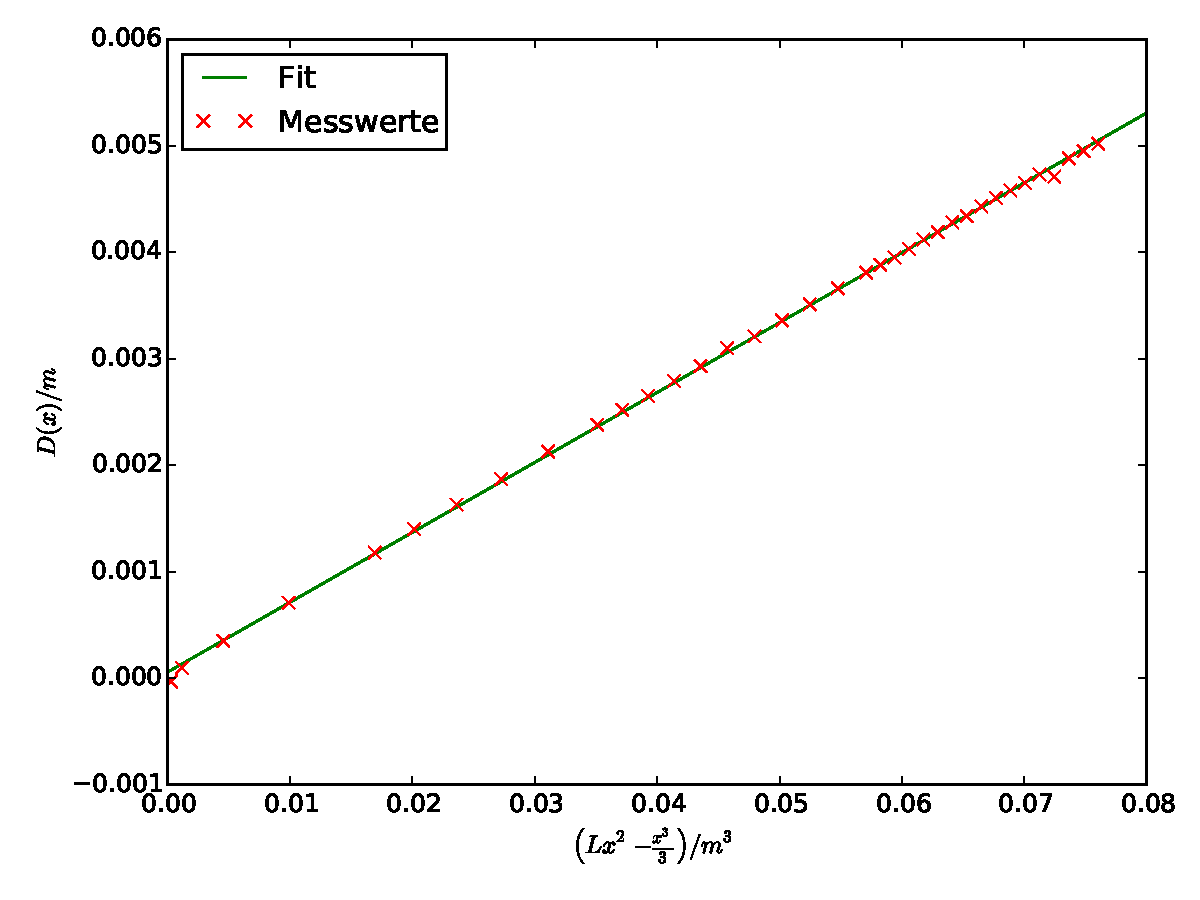
\includegraphics[width=0.9\textwidth]{stab1_einseitig.pdf}
  \caption{Lineare Ausgleichsrechnung für den einseitig eingespannten eckigen Stab.}
  \label{fig:plot_einseitig1}
\end{figure}
\begin{align*}
  a &= \SI{0.0657(2)}{\per\squared\meter} \\
  b &= \SI{0.6(1)e-3}{\meter}.
\end{align*}
Nach Gleichung \eqref{eqn:durchbiegung1} wird der Elastizitätsmodul dann mit
\begin{equation}
  a = \frac{F}{2 E I_1} \iff E = \frac{M_{G1} g}{2 I_1 a}
  \label{eqn:Emodul1}
\end{equation}
bestimmt. Dabei ist $I_1$ das in Abschnitt \ref{sec:Flaechentraegheitsmoment}
berechnete Flächenträgheitsmoment. Für den quadratischen Stab bei einseitiger
Einspannung ergibt sich mit Gaußscher Fehlerfortpflanzung nach Gleichung
\eqref{eqn:fehlerfortpflanzung}, welche mit Python durchgeführt wurde, für den
Elastizitätsmodul folgender Wert:
\begin{align*}
  E = \SI{91.5(3)e+9}{\newton\per\squared\meter}.
\end{align*}


\subsubsection{runder Stab}
Die Messwerte zur Berechnung der Durchbiegung $D(x)$ des runden Stabes bei
einseitiger Einspannung sind in Tabelle \ref{tab:messung2} im Anhang aufgeführt.
Die Masse des Gewichts zur Belastung des Stabes beträgt $M_{G2} = \SI{0.5285}
{\kilo\gram}$, die effektive Länge des Stabes ist wieder $L=\SI{0.49}
{\meter}$. Analog zur Berechnung des Elastizitätmoduls des eckigen Stabes bei
einseitiger Einspannung wird eine lineare Ausgleichsrechnung durchgeführt, welche
in Abbildung \ref{fig:plot_einseitig2} zu sehen ist und auf die Werte
\begin{figure}
  \centering
  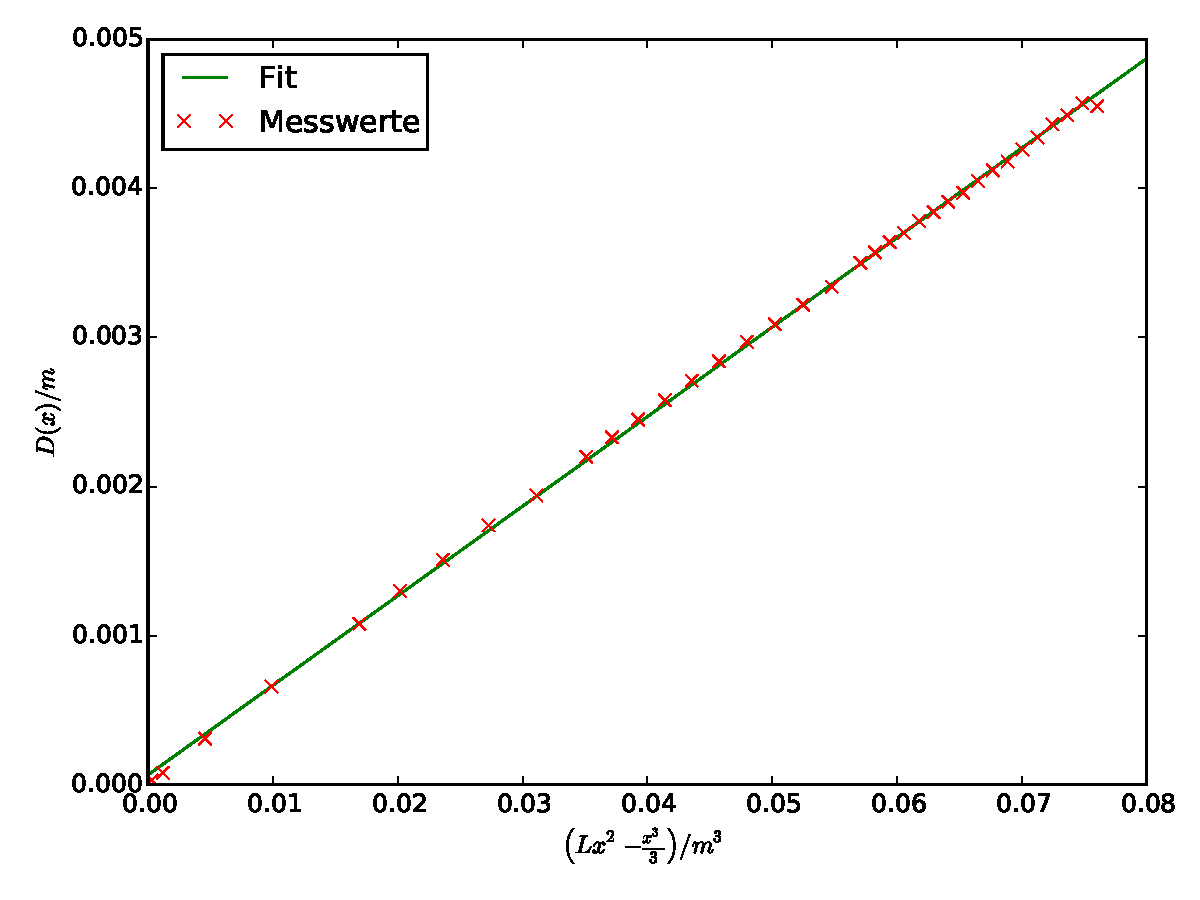
\includegraphics[width=0.9\textwidth]{stab2_einseitig.pdf}
  \caption{Lineare Ausgleichsrechnung für den einseitig eingespannten runden Stab.}
  \label{fig:plot_einseitig2}
\end{figure}
\begin{align*}
  a &= \SI{0.0601(2)}{\per\squared\meter} \\
  b &= \SI{7(1)e-5}{\meter}
\end{align*}
für die Parameter $a$ und $b$ führt. Für den Elastizitätsmodul ergibt sich dann
vergleichbar zu Gleichung \eqref{eqn:Emodul1} jedoch mit dem Flächenträgheitsmoment
$I_2$
\begin{equation}
  E = \frac{M_{G2} g}{2 I_2 a} = \SI{87.9(3)e+9}{\newton\per\squared\meter}.
\end{equation}

\subsection{Beidseitige Einspannung}
Die zur Berechnung verwendeten Messwerte sind im Anhang in Tabelle \ref{tab:messung3a}
und \ref{tab:messung3b} zu finden. Bei der beidseitigen Einspannung ist zu
beachten, dass die Abstände immer von einem Ende des Stabes aus gemessen wurden
und nicht jeweils vom Einspannpunkt bis zur Mitte. Deshalb müssen die Bereiche
$0\leq x \leq \frac{L}{2}$ und $\frac{L}{2}\leq x \leq L$ getrennt berechnet
werden. Die effektive Stablänge bei beidseitiger Einspannung ist $L= \SI{0.553}
{\meter}$, die Masse des angehängten Gewichts $M_{G3} = \SI{4.689} {\kilo\gram}$.

\subsubsection{linke Seite $(0 <= x <= \frac{L}{2})$}
In diesem Fall wird das Polynom $\left(3 L^2 x - 4 x^3\right)$ gegen $D(x)$
aufgetragen und eine lineare Ausgleichsrechnung wie bei der einseitigen Einspannung
durchgeführt. Der Graph ist in Abbildung \ref{fig:plot_beidseitig1} zu sehen.
Für die Parameter $a$ und $b$ erhält man in diesem Fall die Werte
\begin{align*}
  a &= \SI{0.0122(3)}{\per\squared\meter}\\
  b &= \SI{4(4)e-5}{\meter}.
\end{align*}
\begin{figure}
  \centering
  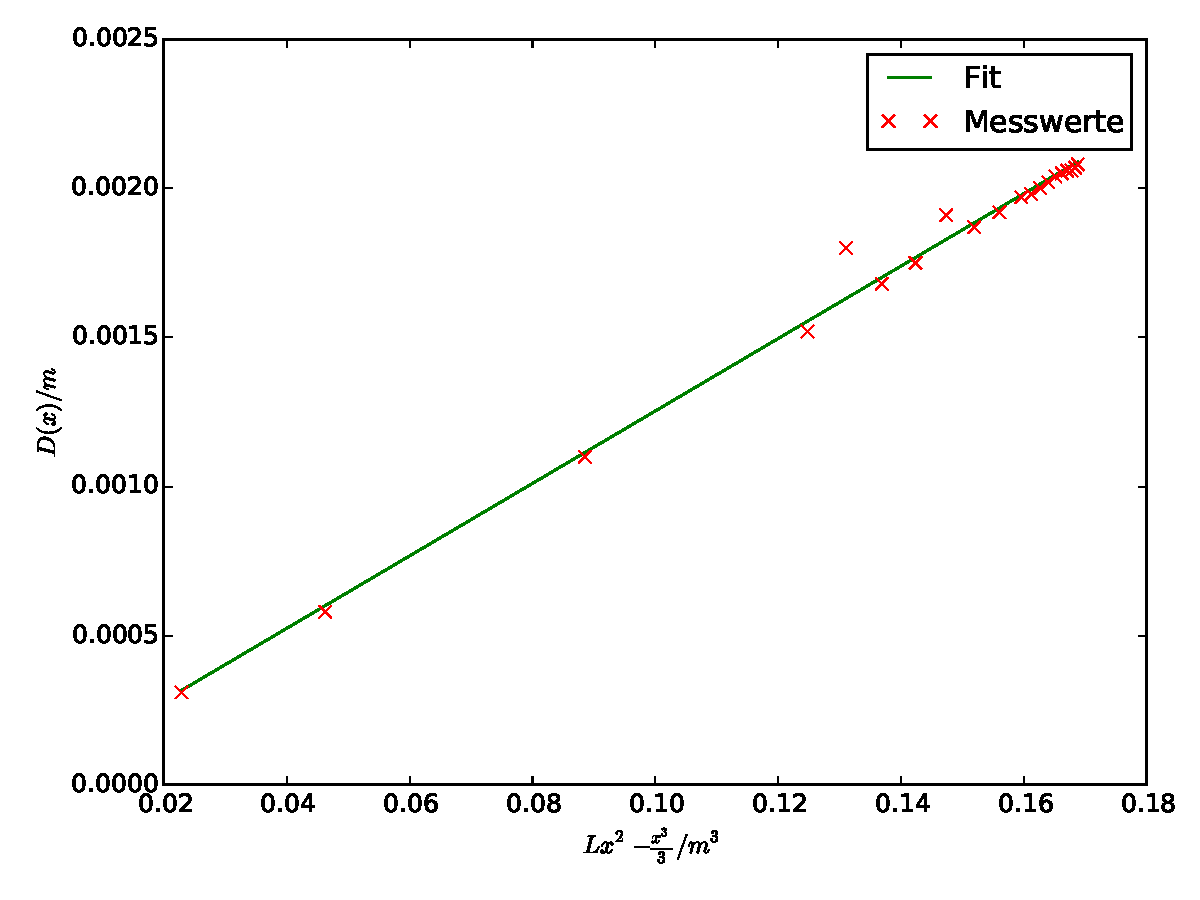
\includegraphics[width=0.9\textwidth]{stab1_beidseitig_links.pdf}
  \caption{Lineare Ausgleichsrechnung für den beidseitig eingespannten eckigen Stab.}
  \label{fig:plot_beidseitig1}
\end{figure}
Für den Elastizitätsmodul folgt nach Gleichung \eqref{eqn:durchbiegung_links}
\begin{equation}
  a = \frac{F}{48 E I_1} \iff E = \frac{M_{G3} g}{48 I_1 a}
  = \SI{95(2)e+9}{\newton\per\squared\meter}
  \label{eqn:Emodul3}
\end{equation}

\subsubsection{rechte Seite $(\frac{L}{2} <= x <= L)$}
Hier wird das Polynom $\left(4 x^3 - 12 L x^2 + 9 L^2 x - L^3\right)$ gegen $D(x)$
aufgetragen und wiederum eine lineare Regression durchgeführt, die die Werte
\begin{align*}
  a &= \SI{0.01207(6)}{\per\squared\meter}\\
  b &= \SI{5(1)e-5}{\meter}
\end{align*}
liefert. Der Graph ist in Abbildung \ref{fig:plot_beidseitig2} dargestellt. Der
Elastizitätsmodul wird sodann mit Gleichung \eqref{eqn:Emodul3} berechnet und ergibt
\begin{align*}
  E = \SI{95.2(4)e+9}{\newton\per\squared\meter}
\end{align*}
\begin{figure}
  \centering
  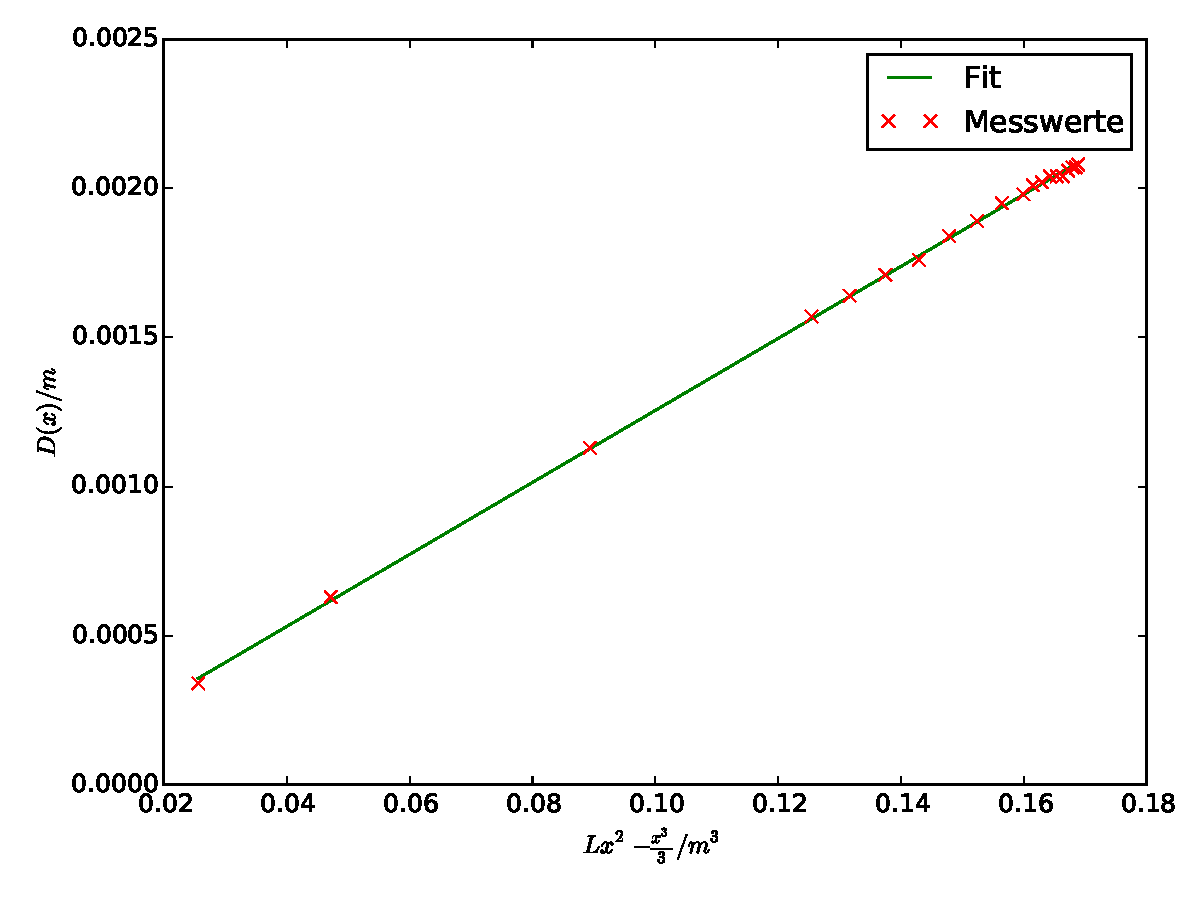
\includegraphics[width=0.9\textwidth]{stab1_beidseitig_rechts.pdf}
  \caption{Lineare Ausgleichsrechnung für den beidseitig eingespannten eckigen Stab.}
  \label{fig:plot_beidseitig2}
\end{figure}

\subsection{Vergleich mit Literaturwerten}
Beide Stäbe bestehen aus Messing. Da die genaue Zusammensetzung der Messinglegierung
jedoch nicht bekannt ist, kann keine relative Abweichung der berechneten
Elastizitätsmoduln angegeben werden. Für Messing ist in der Literatur \cite[275]{geschke}
\begin{align*}
  E_\text{Literatur} &= 80...103\, \si{\giga\newton\per\squared\meter}
  \intertext{angegeben. Alle berechneten Elastizitätsmoduln liegen in diesem Rahmen:}
  E_\text{Stab 1,einseitg} &= \SI{91.5(3)e+9}{\newton\per\squared\meter}\\
  E_\text{Stab 2,einseitg} &= \SI{87.9(3)e+9}{\newton\per\squared\meter}\\
  E_\text{Stab 1,beidseitig1} &= \SI{95(2)e+9}{\newton\per\squared\meter}\\
  E_\text{Stab 1,beidseitig2} &= \SI{95.2(4)e+9}{\newton\per\squared\meter}.
\end{align*}
Bildet man den Mittelwert der drei Elastizitätsmoduln, die für Stab 1 berechnet
wurden, so erhält man $E_\text{Stab 1, mittel} = \SI{93.8(7)e+9}{\newton\per\squared\meter}$
mit einer Standardabweichung von $\SI{1.2(3)e+9}{\newton\per\squared\meter}$.
